<<echo=FALSE, cache=FALSE>>=
set_parent('./project.Rnw')
@
%
To measure the performance and explore the how well theory and practice coincide, the methods discussed will be trained and tested on different datasets in this chapter. Some extensions will also briefly be discussed at the end.

\section{Spam dataset}
\label{sec:Spam dataset}
\colorbox{yellow}{Need to write something about the data set. Description and so on.}\\
\colorbox{yellow}{Look at what others have done.} \\
\url{http://sci2s.ugr.es/keel/dataset.php?cod=109} Spam data.\\
\\
\colorbox{yellow}{If I use categorical variables, should I include section on how the algorithms handles them?}\\
 The first dataset explored is a pretty common dataset in the machine learning world. 
 Each data point in the dataset corresponds to an email, with the binary response telling if an email is spam or not. There are a total of 4601 data points and 57 predictors:
 \begin{itemize}
   \item 48 continuous real $[0, 100]$ corresponding to words. Each giving the percentage of words in the email matching that word. 
   \item 6 continuous real $[0, 100]$ corresponding to characters. Each giving the percentage of characters in the email matching that characters.
   \item 1 continuous real $[1, \ldots]$ giving average length of uninterrupted sequences of capital letters. 
   \item 1 continuous integer $[1, \ldots]$ giving length of longest uninterrupted sequence of capital letters.
   \item 1 continuous integer $[1, \ldots]$ giving total number of capital letters in the email.
 \end{itemize}
 For more information on the dataset see \cite{Spamdata}.

 In the tests that follows the spam data was split into a training and test set of same size. The algorithms are first trained on the training set, and the test error in form of $0/1$ misclassification error rate is plotted, i.e.
 \begin{align}
   \label{eq:missClassErr} 
   error =  \frac{1}{n_{test}} \sum_{i = 1}^{n_{test}} I\{C(\mathbf{x}_i) \neq y_i\},
 \end{align}
 where $C(\mathbf{x}_i)$ is the prediction based on $\mathbf{x}_i$, and $n_{test}$ is the number of test points. If the goal had been to actually make a spam filter, the error measure would not weight misclassification of spam and non-spam the same. Different costs for misclassification has not been the focus of this project, but for the purpose of testing the behavior of different methods \eqref{eq:missClassErr} works well.
\\ 
\\
In all the following experiments, the methods are trained on half the data and tested on the other half. All methods are trained using the same data points. 

\section{CART}
\label{sec:CARTsim}
Simulation 1: \\
Plot test error for different \verb+cp+ parameters, or (same) different pruning. From full tree, back to a stump.\\
\\
First classification trees were fitted to the data using \verb+rpart+ by \cite{rpart}. Large trees was grown using both the Gini index and deviance. They were then pruned back to a single node and the test errors for the different trees were plotted as function of the tree size in Figure~\ref{fig:cartCPSpam}. 
%
\begin{figure}[h!tp]
\begin{center}
    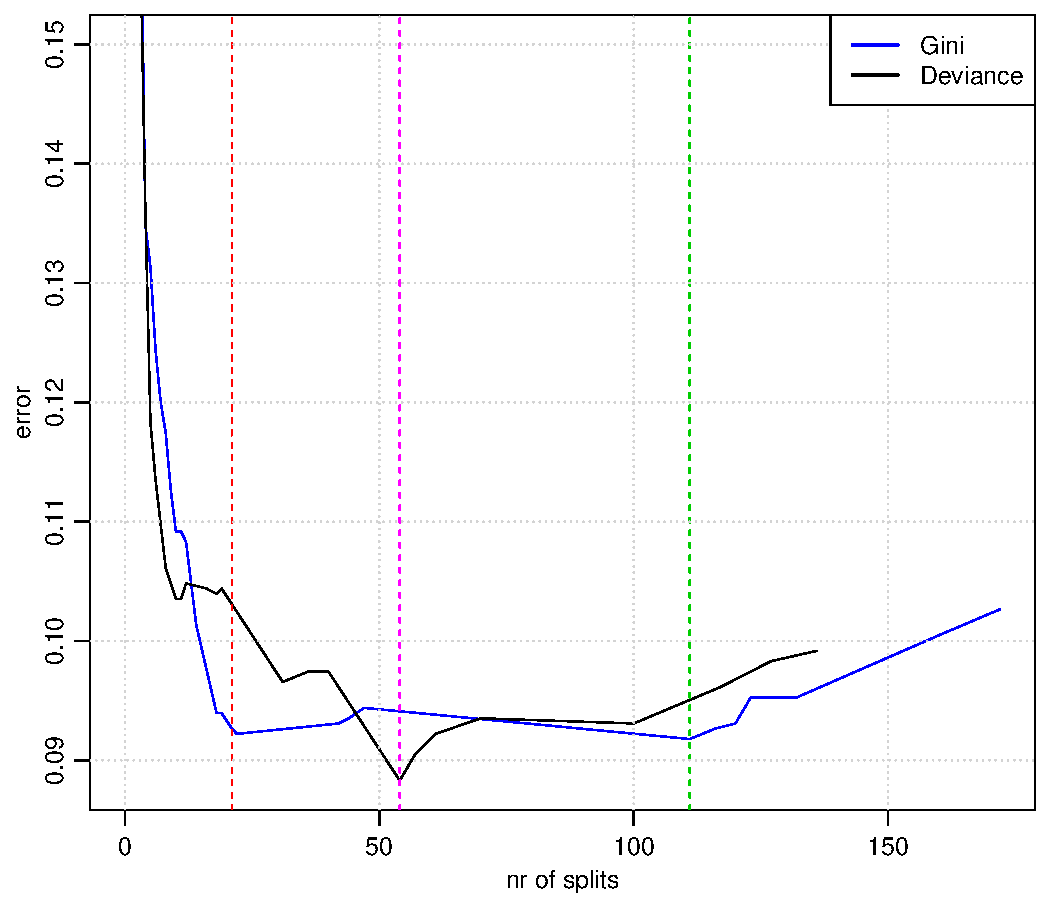
\includegraphics[scale=0.5]{./figures/cartCPSpam.pdf}
\end{center}
\caption{CART on spam data. Test error as function of number of splits. The two lines represent trees grown with Gini index and deviance splitting criterion. A large tree is grown and the different points are test error of pruned trees depending on the tuning parameter $\alpha$ in \eqref{eq:CostPruning}. The green and magenta line marks the minima for the two lines. }
\label{fig:cartCPSpam}
\end{figure}
%
Both methods show how small trees are underfitted while large trees are overfitted, and somewhere in the middle, the optimal tree can be found. 

The green line marks the minimum test error using the Gini index. This graph is very flat around the minimum, so in terms of interpretability, a smaller tree can be chosen without sacrificing much of the predicting power. In Figure~\ref{fig:CartSpam}, the optimal tree (green) is displayed along the tree from the red line. Their performance is almost identical, but the red tree give a nicer view of the data. Usually the trees are plotted with the splits like in Figure~\ref{fig:cart}. Here, they are left out because they serve no purpose in the context of the experiment. If the goal was to find which factors were most important in terms of classifying spam, they would be investigated more closely.

The magenta figure in Figure~\ref{fig:CartSpam}, is the tree grown using deviance in Figure~\ref{fig:cartCPSpam} corresponding to the magenta line.In this experiment, it outperforms all the Gini trees, though only barely. 

\begin{figure}[h!tp]
  \centering
  \begin{subfigure}[b]{0.48\textwidth}
    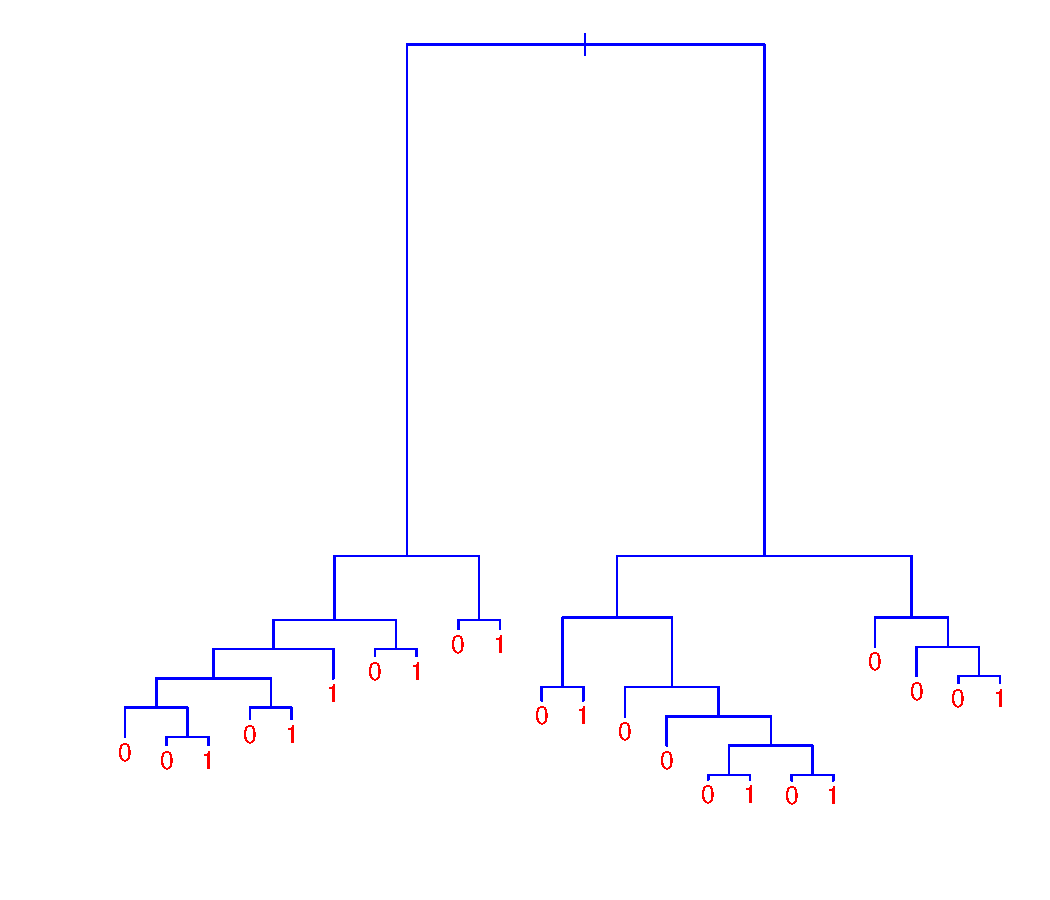
\includegraphics[width=\textwidth]{./figures/cartSmallSpam.pdf}
  \end{subfigure}%
  \quad
  \begin{subfigure}[b]{0.48\textwidth}
    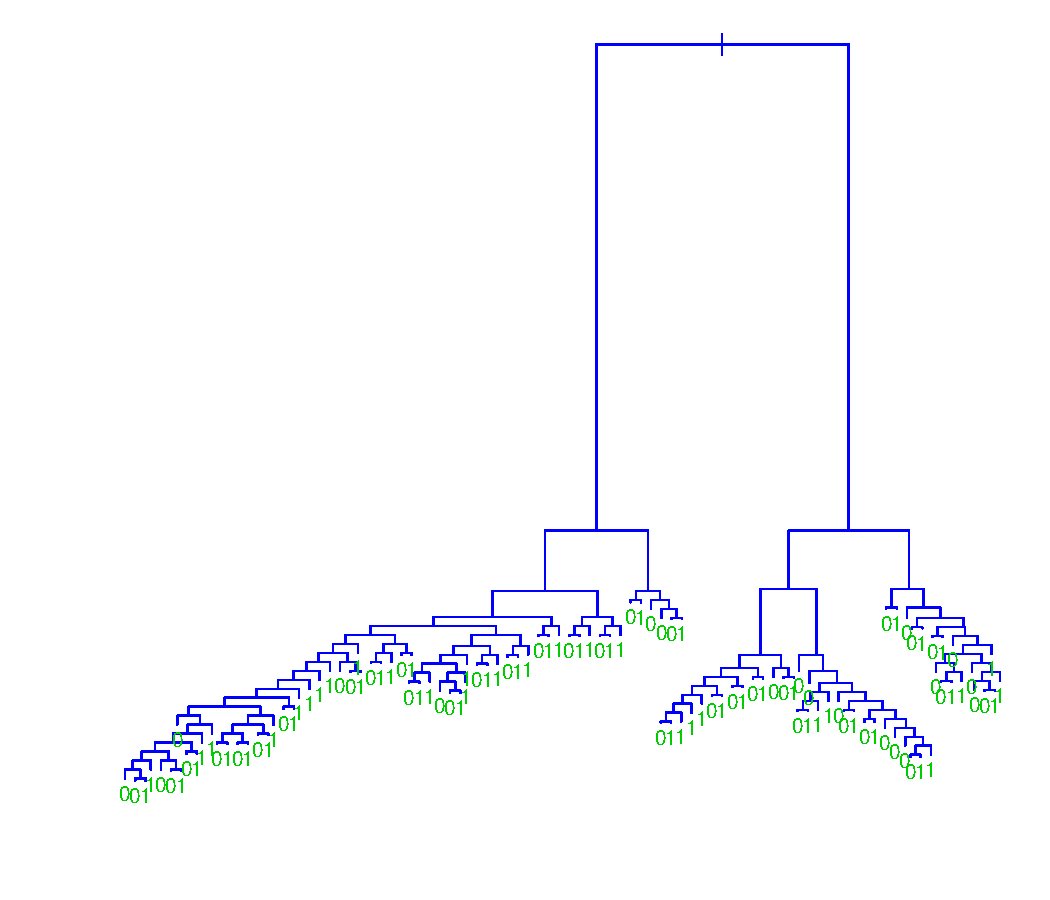
\includegraphics[width=\textwidth]{./figures/cartOptSpam.pdf}
  \end{subfigure}
  \quad
  \begin{subfigure}[b]{0.48\textwidth}
    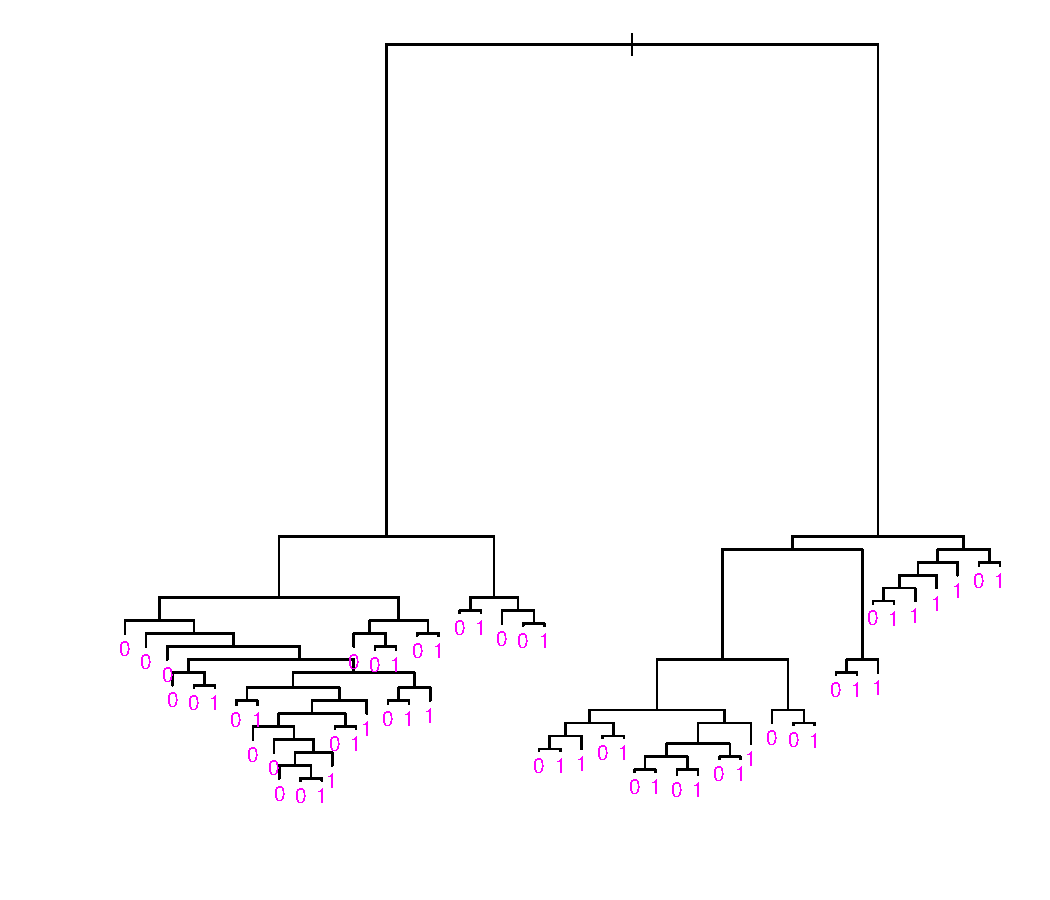
\includegraphics[width=\textwidth]{./figures/cartOptDevianceSpam.pdf}
  \end{subfigure}
          %(or a blank line to force the subfigure onto a new line)
  \vspace{1\baselineskip}
  \caption{CART on spam data. Trees from \ref{fig:cartCPSpam} are displayed. The green tree has the minimal test error using the Ginie index, while the red have a much simpler structure with almost the same test error. The magenta tree is the best performing using the deviance splitting criterion.}
  \label{fig:CartSpam}
\end{figure}
\colorbox{yellow}{Write something about how the red tree is the same as the green tree only with more nodes collapsed.}\\




\section{Adaboost}
\label{sec:SimAdaBoost}
Adaboost was fitted to the spam data using the package \verb+adabag+ by \cite{adabag}. It use the \verb+rpart+ implementation of CART in Section~\ref{sec:CARTsim} as base classifiers. The main tuning parameters in Adaboost is the number of iterations, and the tree depth. In Figure~\ref{fig:adaboostSpam}, the test error is plotted as function of iterations, for different tree depths. It is clear that the algorithm does pretty well after few iterations, and outperforms CART easily. Only a maximum of 300 iterations were done, but by the look of it, Adaboost seems quite robust to overfitting. 

Surprisingly, Adaboost does better for deeper trees. It is expected to overfit for larger trees, but it does not. One possible explanation could be that there is higher order interactions between the features in the dataset. It is not possible to fit trees deeper than $30$ in the \verb+adabag+ package, but it would have been interesting to see how the performance developed for even deeper trees.
%
\begin{figure}[h!tp]
\begin{center}
    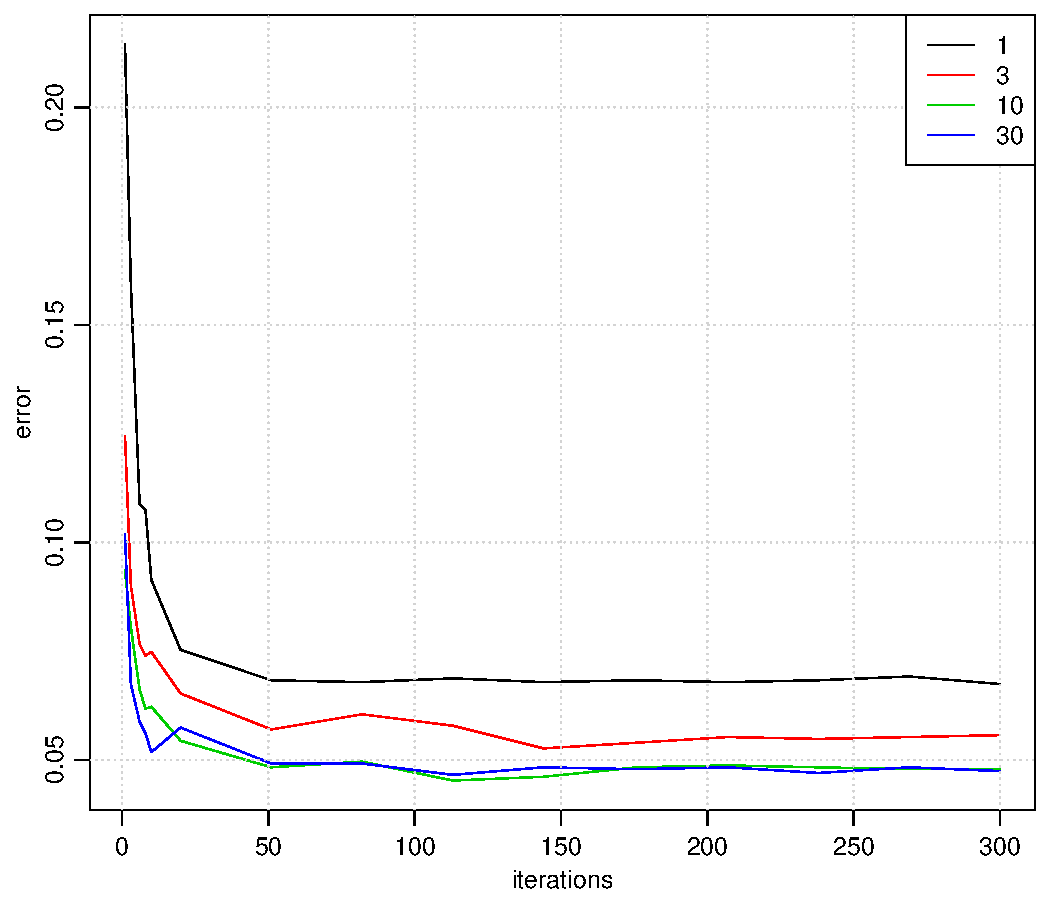
\includegraphics[scale=0.5]{./figures/adaboostSpam.pdf}
\end{center}
\caption{Adaboost on spam data. Each line represent a tree depth.}
\label{fig:adaboostSpam}
\end{figure}
%
\section{Gradient boosting}
\label{sec:SimGradBoost}
Gradient boosting is a very powerful method, but requires a lot of tuning. The goal here was not to find the optimal tuning parameters for the spam dataset, but rather to investigate the effect of changing different parameters. The package \verb+gbm+ by \cite{gbm} was used to fit the gradient boosting with deviance loss.

\begin{figure}[htbp]
  \centering
  \begin{subfigure}[b]{0.48\textwidth}
    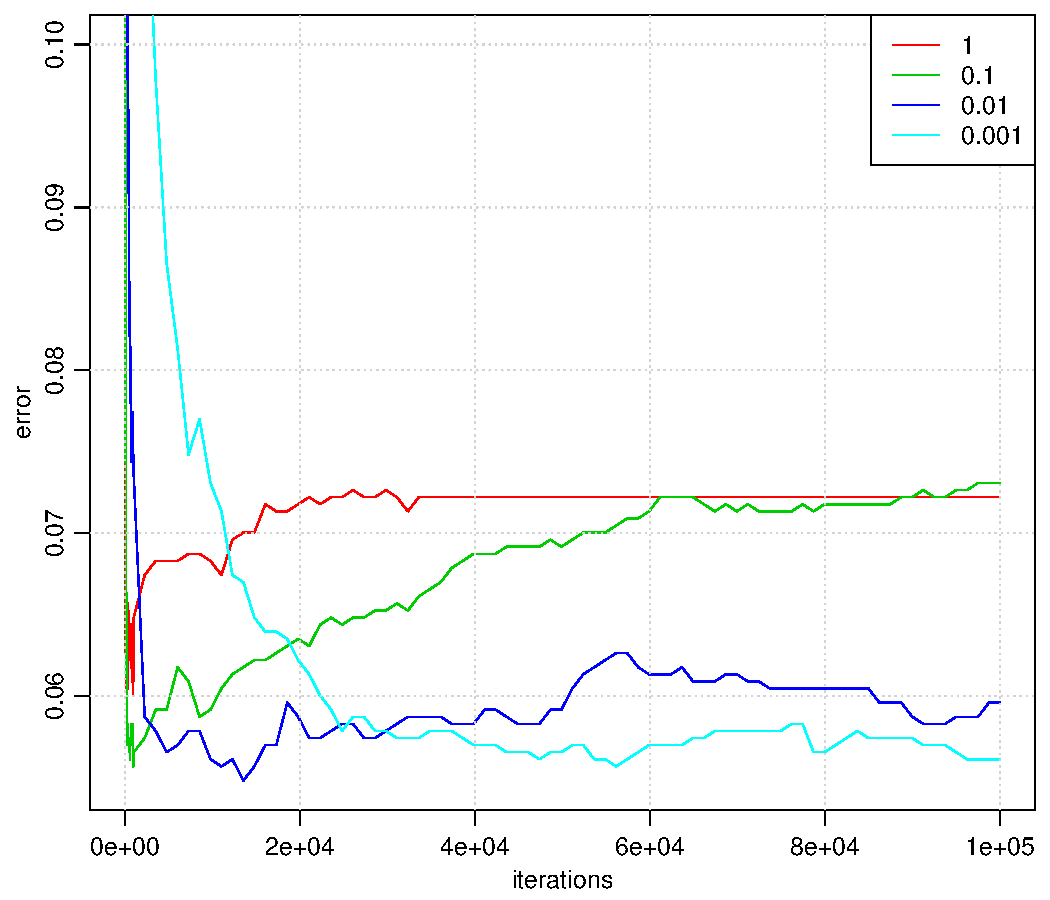
\includegraphics[width=\textwidth]{./figures/gradboostSpamShrink2.pdf}
    \caption{Different shrinkages $\nu$.}
    \label{fig:gradboostSpamShrink2}
  \end{subfigure}%
  \quad
  \begin{subfigure}[b]{0.48\textwidth}
    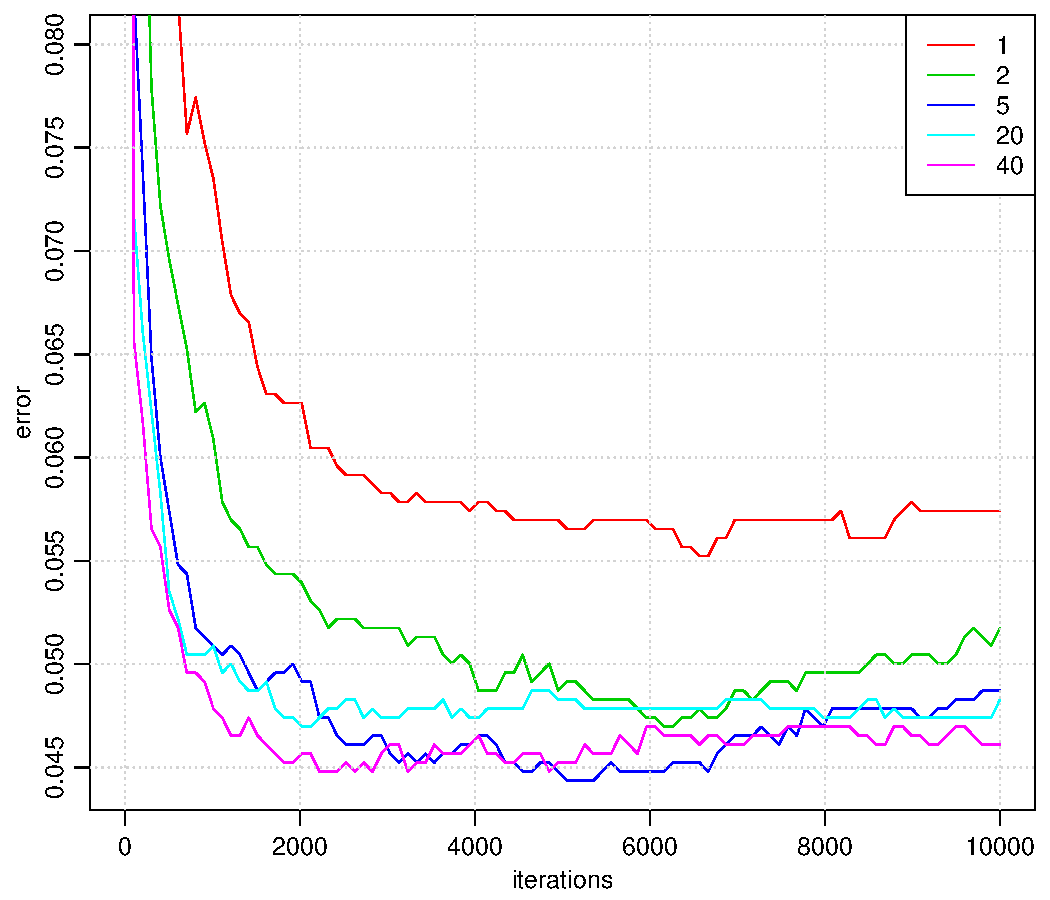
\includegraphics[width=\textwidth]{./figures/gradboostSpamDepth.pdf}
    \caption{Different tree depths.}
    \label{fig:gradboostSpamDepth}
  \end{subfigure}
          %(or a blank line to force the subfigure onto a new line)
  \vspace{1\baselineskip}
  \caption{Gradient boosting on spam data.}
  \label{fig:GradBoostSpam}
\end{figure}

The optimal number of iterations is highly dependent on the shrinkage parameter (see Section~\ref{sub:Shrinkage}). In Figure~\ref{fig:gradboostSpamShrink2} the test error is plotted against number of boosting iterations. Each line represent a different shrinkage. It is clear from the plot that for lower shrinkage, the number of iteration needed increase. This mean shrinkage comes as a cost in terms of computations. However, the worst performing line is that without shrinkage ($\nu = 1$), although not a very large difference. In this case it seems like the is no point with $\nu < 0.1$ as there is no gain in test error.

It is also clear form the plot that gradient boosting can overfit, but note that many iterations are needed, so there is no evidence that it is less robust than Adaboost.

As with Adaboost, the depth of the trees plays an important role. In Figure~\ref{fig:gradboostSpamDepth} test error for different tree depths are displayed. \verb+gbm+ does not take depth as a parameter, but a parameter called \verb+interaction.depth+, which represent the interactions in Section~\ref{sub:Tree size}. $1$ is an additive model, $2$ is a model with up to second order interactions. In principle \verb+interaction.depth+$+1$ gives the maximum number of terminal nodes.

The figure show the same trend as Adaboost did. Deeper trees give better results, although the difference is much smaller for gradient boosting.
\\
%
\begin{figure}[htbp]
\begin{center}
    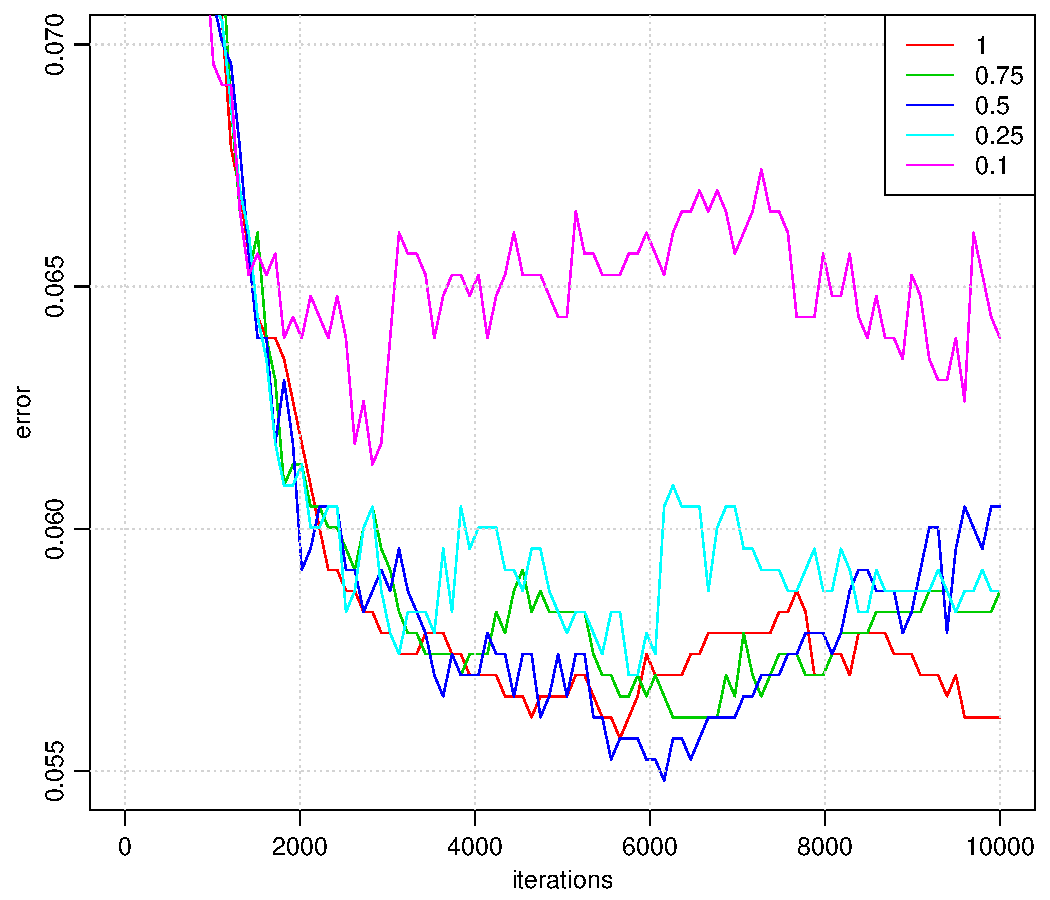
\includegraphics[scale=0.5]{./figures/gradboostSpamStoch.pdf}
\end{center}
\caption{Stochastic gradient boosting on spam data. The bootstrap fractions are specified in the legend.}
\label{fig:StochasticGradBoost}
\end{figure}
\\
Stochastic gradient boosting was mentioned as a small modification of gradient boosting in Section~\ref{sub:Stochastic gradient boosting}. The only difference is that a subset of the training data is drawn (without replacement) at each iteration. \verb+gbm+ refers to this parameter as the \verb+bag.fraction+. In Figure~\ref{fig:StochasticGradBoost}, the test error is plotted for different bootstrap fractions. From the figure is looks like there is little gain in error from introducing randomness. However, for bootstrap fractions down to $0.5$ the performance is not worse. As a smaller dataset requires less computations, there is still some gain in doing stochastic gradient boosting here.

\section{Bagging and Random Forest}
\label{sec:BaggandRFSim}
Simulation 1: \\
Do simulations for bagging with different bootstrap sizes. And the same for random forests\\
\\
\begin{figure}[h!]
  \centering
  \begin{subfigure}[b]{0.48\textwidth}
    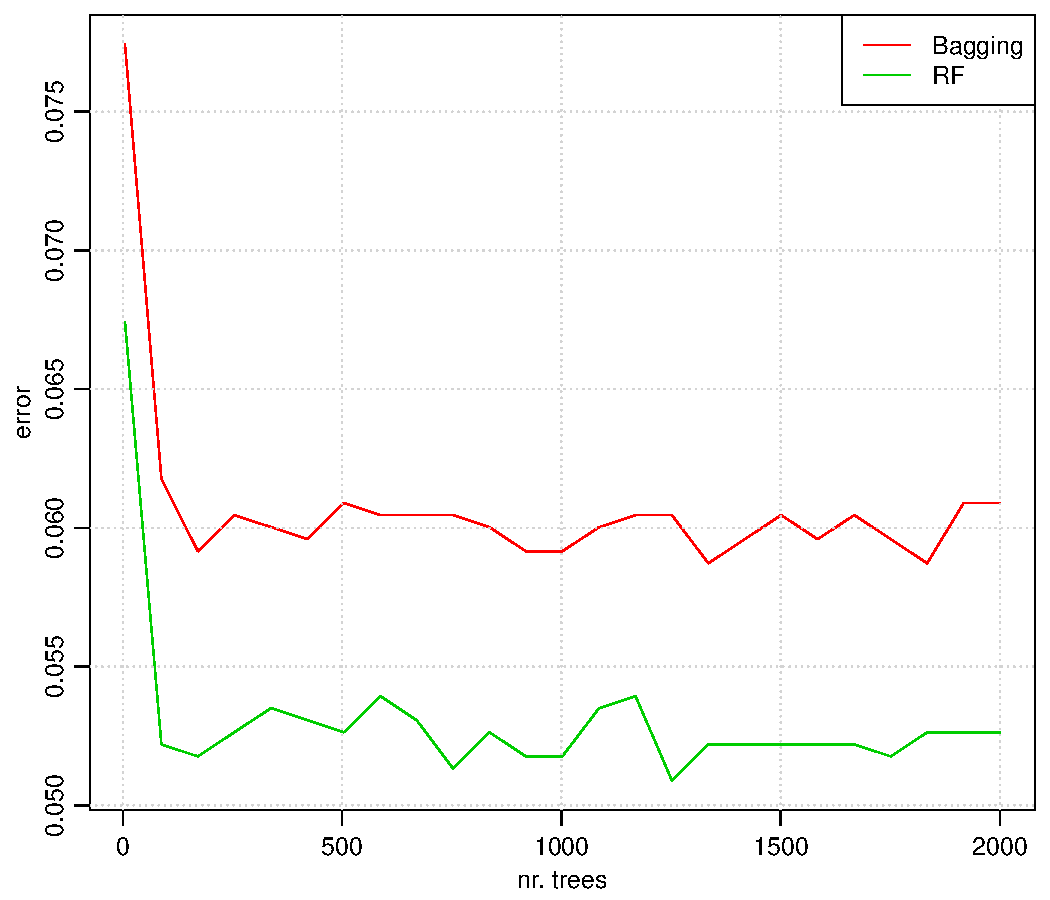
\includegraphics[width=\textwidth]{./figures/baggingAndRFSpam.pdf}
    \caption{Test error as function of bootstrap samples for bagging and RF.}
    \label{fig:baggingAndRFSpam}
  \end{subfigure}%
  \quad
  \begin{subfigure}[b]{0.48\textwidth}
    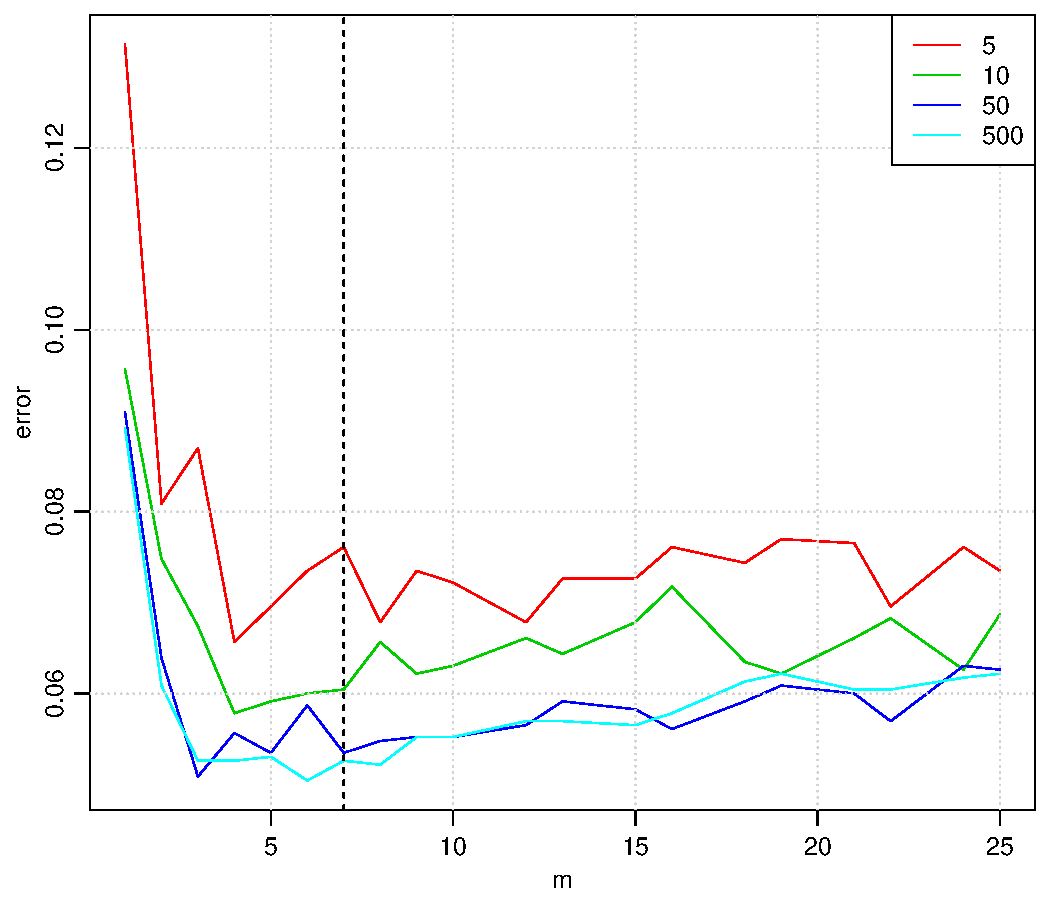
\includegraphics[width=\textwidth]{./figures/RFSpam.pdf}
    \caption{RF as func. of m, for different number of bootstrap samples. Vertical line marks $\sqrt{p}$.}
    \label{fig:RFSpam}
  \end{subfigure}
          %(or a blank line to force the subfigure onto a new line)
  \vspace{1\baselineskip}
  \caption{Misclassification rate for bagging and random forests on spam data.}
  \label{fig:baggAndRF}
\end{figure}
\todo{Comment on line in Figure~\ref{fig:RFSpam}}
\colorbox{yellow}{Comment how Figure~\ref{fig:baggingAndRFSpam} is many runs and not different iterations for one run.}
\\\colorbox{yellow}{That is why it is not smooth compared to Figure~\ref{fig:OOBvsTestvsCV}.}


Simulation 2: \\
\\
Maybe together with bagging, do simulations for as function of $m$'s, for different bootstrap sizes? \\
\colorbox{yellow}{Not sure what is best here.}\\
\\
\colorbox{yellow}{Comment that Figure~\ref{fig:baggingAndRFSpam} shows how RF don't overfit. Is the same true for bagging?}\\
\\
Simulation 3: \\
Show an example of when bagging and RF fails? If the base classifier is bad, then the aggregated can be bad as well.\\
\colorbox{yellow}{Should I do this?}\\
\\
\colorbox{yellow}{Do simulation to show diffenece between \eqref{eq:aggClass} and \eqref{eq:aggClassP}.}


\begin{figure}[h!]
\begin{center}
    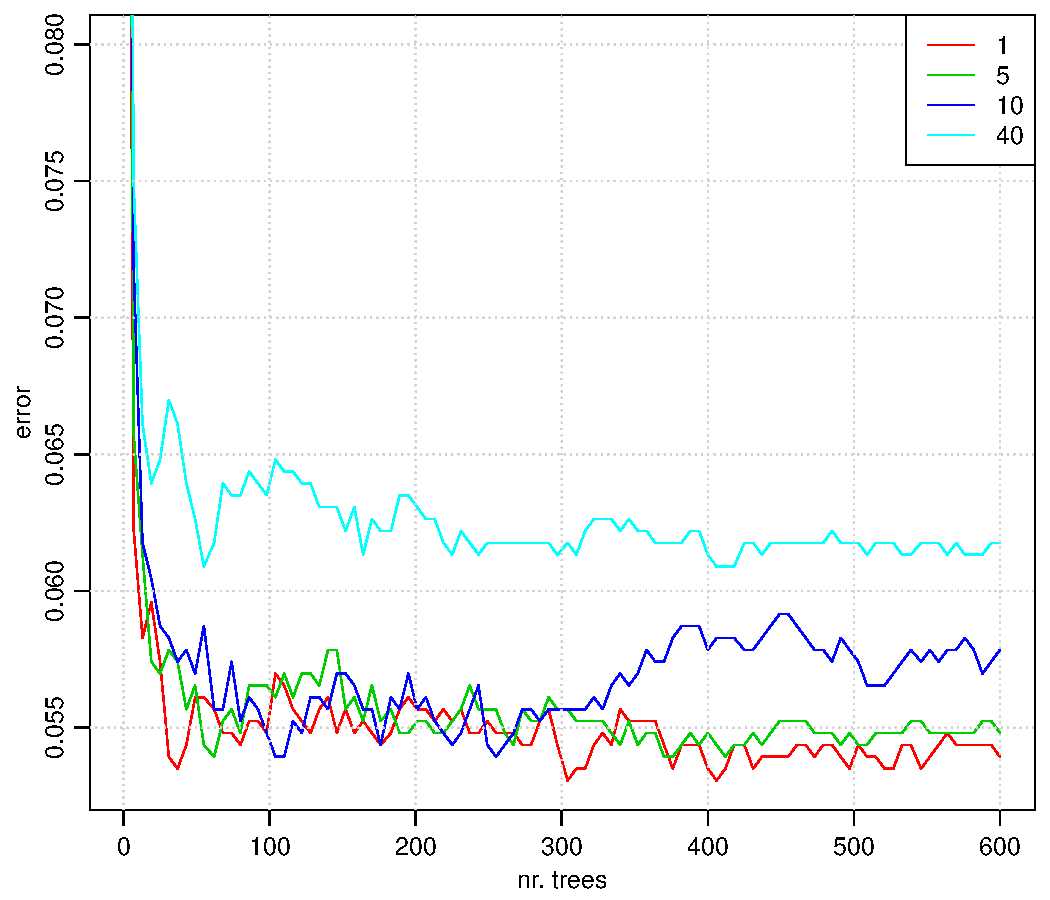
\includegraphics[scale=0.5]{./figures/RFTreeDepth.pdf}
\end{center}
\caption{Random forest on spam data, with different tree depths. The numbers in the legend indicates the minimum number of nodes in a terminal node.}
\label{fig:RFTreeDepth}
\end{figure}
\colorbox{yellow}{Benefits of not growing full sized trees is that it is faster, and some regularization.}


\begin{figure}[h!]
\begin{center}
    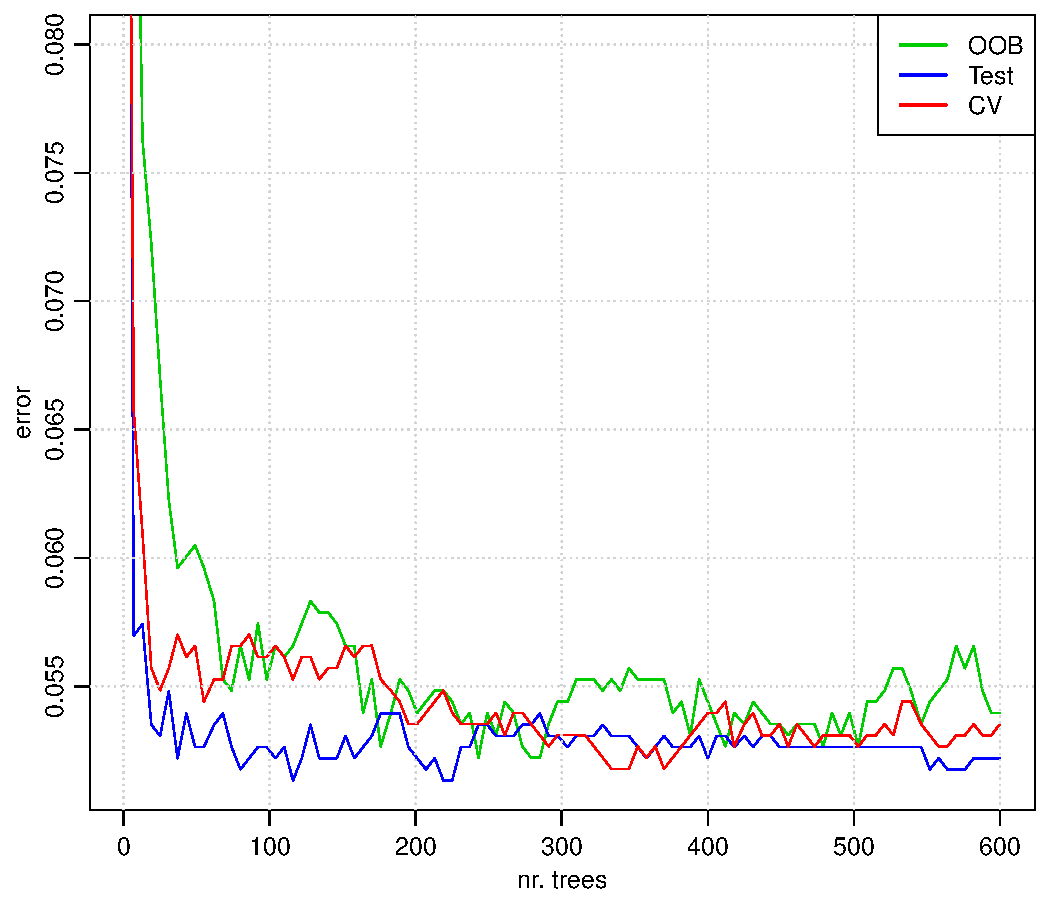
\includegraphics[scale=0.5]{./figures/OOBvsTestvsCV.pdf}
\end{center}
\caption{Out-of-bag, 10-fold cross-validation and test error for random forest on spam data.}
\label{fig:OOBvsTestvsCV}
\end{figure}
\colorbox{yellow}{Comment how they are very random, so Figure~\ref{fig:OOBvsTestvsCV} varies a lot.}\\






\section{Compare methods}
\label{sec:Compare methods}
\colorbox{yellow}{Show CART here as well.}

\subsection{Robustness}
\label{sub:Robustness}

\colorbox{yellow}{Add noise to previous test and see how stable the results are.}
\section{Phoneme}
\label{sec:Phoneme}
\begin{figure}[h!]
\begin{center}
    \includegraphics[scale=0.5]{./figures/cartCPPhoneme.pdf}
\end{center}
\caption{CART on Phoneme data.}
\label{fig:cartCPPhoneme}
\end{figure}


\begin{figure}[h!]
\begin{center}
    \includegraphics[scale=0.5]{./figures/adaboostPhoneme.pdf}
\end{center}
\caption{Adaboost on Phoneme data. For different tree depths.}
\label{fig:adaboostPhoneme}
\end{figure}

\begin{figure}[h!]
\begin{center}
    \includegraphics[scale=0.5]{./figures/gradboostPhonemeShrink2.pdf}
\end{center}
\caption{Gradient boosting on Phoneme data. The shrinkage of each line is specified in the legend.}
\label{fig:gradboostPhonemeShrink2}
\end{figure}

\begin{figure}[h!]
  \centering
  \begin{subfigure}[b]{0.48\textwidth}
    \includegraphics[width=\textwidth]{./figures/gradboostPhonemeStoch.pdf}
    \caption{Different bootstrap fractions.}
    \label{fig:gradboostPhonemeStoch}
  \end{subfigure}%
  \quad
  \begin{subfigure}[b]{0.48\textwidth}
    \includegraphics[width=\textwidth]{./figures/gradboostPhonemeDepth.pdf}
    \caption{Different tree depths.}
    \label{fig:gradboostPhonemeDepth}
  \end{subfigure}
          %(or a blank line to force the subfigure onto a new line)
  \vspace{1\baselineskip}
  \caption{Stochastic gradient boosting on Phoneme data. Give some parameter values here!!!}
  \label{fig:StochasticGradBoostPhoneme}
\end{figure}

\begin{figure}[h!]
  \centering
  \begin{subfigure}[b]{0.48\textwidth}
    \includegraphics[width=\textwidth]{./figures/baggingAndRFPhoneme.pdf}
    \caption{Test error as function of bootstrap samples for bagging and RF.}
    \label{fig:baggingAndRFPhoneme}
  \end{subfigure}%
  \quad
  \begin{subfigure}[b]{0.48\textwidth}
    \includegraphics[width=\textwidth]{./figures/RFPhoneme.pdf}
    \caption{Test error for RF as function of m, for different number of bootstrap samples. Vertical line marks $\sqrt{p}$.}
    \label{fig:RFPhoneme}
  \end{subfigure}
          %(or a blank line to force the subfigure onto a new line)
  \vspace{1\baselineskip}
  \caption{Misclassification rate for bagging and random forests on Phoneme data.}
  \label{fig:baggAndRFPhoneme}
\end{figure}


\clearpage
\section{Needs to be done}
\label{sec:Needs to be done}
Do bagging/RF with probs instead of vote. (The two different methods in Bagging section). Write something about how p should be faster for B around 0.5.\\
\\
Write about categorical variables after simulation study. In modstat 9.2.4. discussion for CART\\
\\
Comment on how the timing is not particularly good. \\
\\
Comment on how a tree can be deep, but split on the same variable multiple times?\\
\\
Maybe repeat some of experiments with added noise?\\
\\
Find convention on capitalization. Logistic regression, logistic regression, Logistic Regression. \\
Both in text and in section names.\\
\\
Clean up code so everything after quit is removed\\
\\
Check that equations are correct\\
\\
Random forests or Random forest? \\
\\
Find first reference to cross-validation, and write section in appendix.\\
\\



\section{Questions}
\label{sec:Questions}
Need to borrow book again. \\
\\
How much should be explained in the simulation part? Give all inputparameters?\\
\\
How does linear classifier fit into this project?\\
\\
Should the bias-variance tradeoff be descussed before CART (as now), or inside the CART section?\\
\\
Should I call it Simulations, or Numerical experiments, or somehting else? (Just experiments?)\\
\\
Should I have Preface, abstract (also in norwegian), Project overview?\\
\\
Should Linear classifiers be a seperate chapter? \\
\\
Should all methods Boosting, Bagging, RF get their own chapter?\\
\\
Should the derivations of "Why random forest work" be put in the appendex, and only the idea and results discussed in that section?\\
\\
Should I remove the equation number on equations note referred to?\\
\\
Preface and abstract.\\
\\
Where should the notation section be? \\
\\
Should I remove section about computation time in the introduction? \\
\\
Ordered classes in introduction.\\
\\
Should i mention for Logistic regression that by regularizing it it pretty powerfull? And that QDA and RDA exist aswell?\\
\\
Do simulations on importance of training set size? \\
\\
Need book to do the Fisher's linear discriminant sectino\\
\\
Should I look into randomized Adaboost? \cite{freund1996}. I think it's called boosting by resampling. In \verb+adabag+ I think they call it bootstrapping.\\
\\
In boosting experiments, should I specify input parameters in the different plots? \\
\\
Is argument for why votes does not give probailities good? In Bagging.\\
\\
Conclusion and Suggestions for further work?\\
\\
Discussion?\\
\\
